\documentclass[12pt,a4paper]{article}
\usepackage[a4paper]{geometry}
\usepackage{array}
\usepackage{hhline}
\usepackage{csvsimple}
\usepackage[russian,english]{babel}
\usepackage[utf8]{inputenc}
\usepackage[T2A]{fontenc} 
\usepackage{ulem}
\usepackage{cmap}
\usepackage{makecell}
\usepackage{ifpdf}
\usepackage{graphicx}
\usepackage{wrapfig}
\usepackage[hidelinks]{hyperref}

\setlength\extrarowheight{2pt}
\setlength{\parindent}{0cm}
%
\newcommand{\phylentry}[6] {\\\hline\makecell{
#1\medskip\\
\hhline{|-|}
\\#2\\#3\medskip\\
\hhline{|-|}\\
{#6}}
&\makecell{#4}&\makecell{#5}}
%Syntax: \phylentry{Who}{When}{Where}{Phylosophy}{NotPhylosophy}{ETC} // currently ETC is not used
\hoffset -1.6cm 
\textwidth  16.5cm 
\textheight 24cm 
%\topmargin -1cm 
\parskip 8pt 
\setlength{\unitlength}{1cm}
\sloppy
\addto\captionsenglish{
\renewcommand{\contentsname}{{\bf CO}ntents}
\renewcommand{\refname}{Bibliography}
\renewcommand{\figurename}{Figure}
\renewcommand{\tablename}{Table}
\renewcommand{\abstractname}{Abstract}
\renewcommand{\partname}{Section}
\renewcommand{\bottomfraction}{0.5}
\renewcommand{\floatpagefraction}{0.4}
\renewcommand{\textfloatsep}{0.5cm}
\renewcommand{\intextsep}{0.6cm}
\renewcommand{\floatsep}{0.3cm}
}

\renewcommand\theadalign{cb}
\renewcommand\theadfont{\bfseries}
\renewcommand\theadgape{\Gape[4pt]}
\renewcommand\cellgape{\Gape[4pt]}
%<pics>
\newcommand{\materialist}[0]{\includegraphics{dummy-achievement.png}}%</pics>



\usepackage{float}
\begin{document}
%..................................................................
\begin{titlepage}
\par 
\vspace*{-2cm}
\begin{center}
{\sf \Large
\vspace*{1.5cm}
{\Huge Семенов, 10-й семестр, 2018 }\\
{Наконец, философия без истории, а не история философии и не философия истории}}\\
\vspace*{2cm}
\scalebox{1.2}{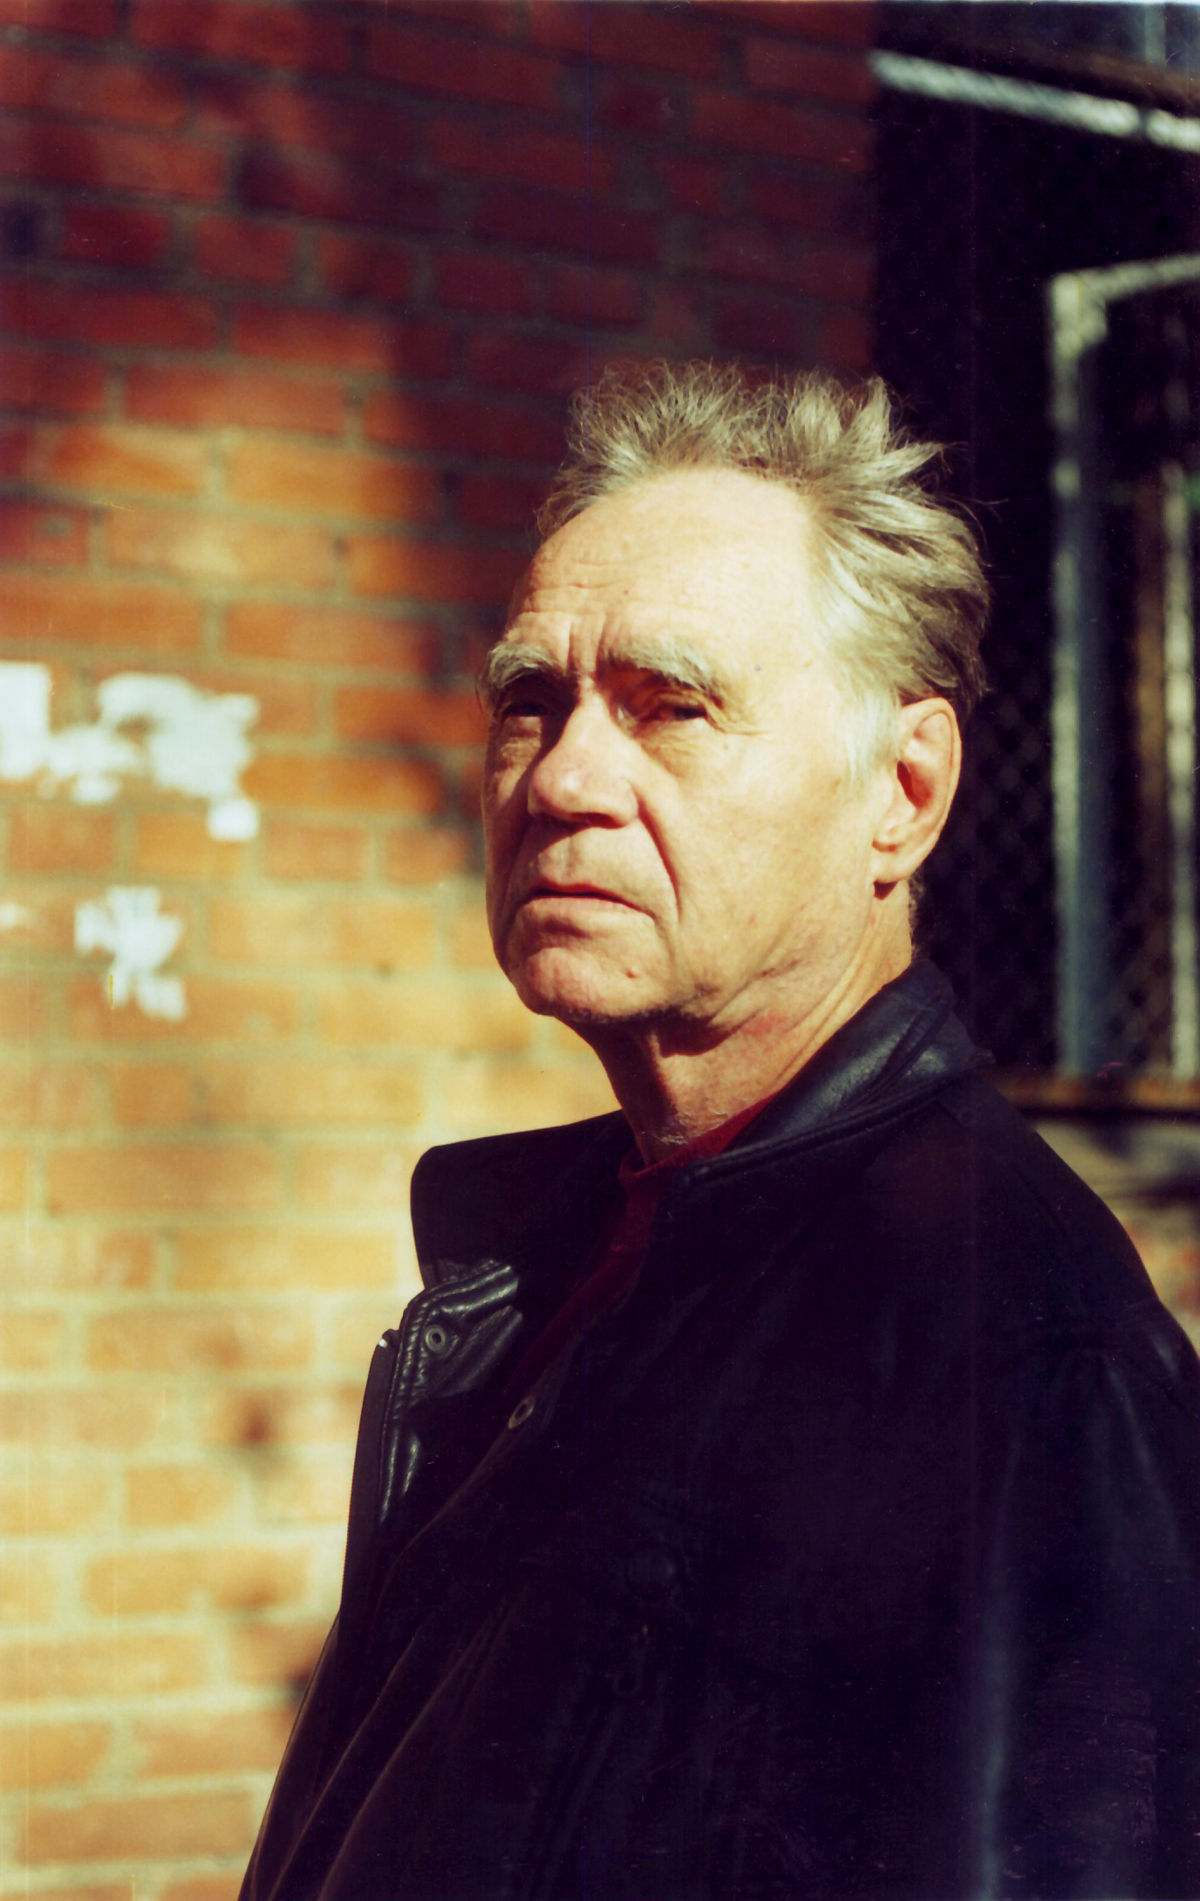
\includegraphics{thegod.png}} 
\begin{flushright}
\sl\small
by Nyaxx11k\\
\end{flushright}
\begin{flushleft}
\hspace{20pt}\raisebox{-33pt}{\scalebox{0.2}{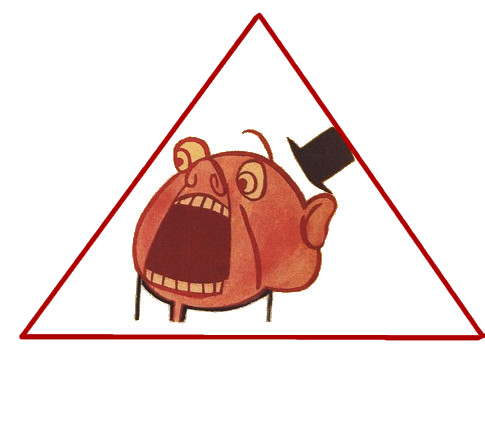
\includegraphics{bourgeois.png}}}
{\itshape Содержит марксизм}
\end{flushleft}
\end{center}
\end{titlepage}
%..................................................................
\topmargin -1cm 
\hoffset -0.7in 
\textwidth 6.0in 
\textheight 9.0in 
\normalsize 
\pagenumbering{arabic}
%----------------
\tableofcontents
%----------------

\section{ Философия как наука об истине, теория познания и самый общий метод исследования.}
Итак, что же такое философия? Если в двух (в четырех) словах, то \textbf{философия} - это наука об истине. \textit{Конечно, любая наука - это об истине (теология - не наука). Но философия - наука об истине в том же смысле, что и биология - наука о живых организмах. Философия ищет истину об истине.} А что мы можем сказать об истине? \textbf{Истина} - это то, что согласуется с действительностью, соответствие между миром и сознанием. Это \textbf{классическое определение истины}. Философия же изучает, как достичь истины, а не заблуждения (\textit{Еще раз, избалованные матлогикой читатели: антипод истины - это заблуждение. Ложь же есть намеренное введение в заблуждение.}). А значит, философия изучает познание, то есть является теорией познания, и она же разрабатывает наиболее общий метод познания, то есть она - наука об этом методе, методология познания. Познание же имеет две ступени - чувственное и мышление. Разрабатывать метод имеет смысл только для второго, ибо первое - это ко врачам. Значит, философия дает наиболее общий метод мышления. Т.е. она еще и наука о наиболее общем методе мышления - \textbf{логика}. Но она же является и самими наиболее общими методами познания и мышления! А еще она онтология. Но это уже третий вопрос. Ибо для него потребуется \textbf{основной вопрос философии}.

\section{ Основной вопрос философии.}
Сразу же ответим: \textbf{"Что первично - мир или сознание?"} Но, спрашивается, почему же он основной? Все дело в том, что мир и сознание надо аккуратно определить - интуитивно-то они и дураку очевидны. Определение дается обычно через род и видовое отличие - "Студент - учащийся (род) высшего учебного заведения (видовое отличие)", "Петух - самец (видовое отличие) курицы домашней (род)". Мир и сознание - два предельно общих понятия, еще более общее - это \textbf{бытие}. Оно включает все. Поэтому содержание утверждения "что-то есть бытие" - это ничто (\textit{Да, про Гегеля правильно вспомнили}). Поэтому так определить мир и сознание нельзя. Можно определить только оба разом, показав отношение между ними. Мир первичен, сознание вторично. Но это у \textbf{материалистов}. Есть еще \textbf{идеалисты}, у которых первично сознание. Причем их три типа - в зависимости от того, б-жественное, мое или общественное сознание в основе всего. Есть еще \textbf{агностики} (хз что первично), \textbf{дуалисты} (оба первичны), \textbf{плюралисты} (много первичного), \textbf{терциалисты} (оба вторичны, а первично что-то третье). \textit{Еще есть те, кто отрицает основной вопрос. Это лжефилософы.} Да, далее нам потребуются термины \textbf{субстанция} и \textbf{акциденция}. Первое - это вещь, которая для существования ни в какой другой вещи не нуждается (\textit{мир/мозг/флешка/кошка (такая-то)}), второе - это то, что существует не само по себе, а в чем-то отличном от него (\textit{сознание как порождение мозга/философия как теория в сознании человека, которое есть продукт мозга/установочный образ линуха на флешке/кошка, но не конкретный Барсик или Мурзик, а кошка вообще}).

\section{ Философия как мировоззрение (онтология). Натурфилософия. Социальная философия (философия истории).}
А раз философия отвечает на главвопрос, то она же дает наиболее общую картину бытия, т.е. является \textbf{мировоззрением} ака \textbf{онтологией}. Раньше еще была \textbf{натурфилософия}. Она пыталась дать наиболее общую картину природы, когда все эти физики/химии только зарождались. В чем-то даже угадала (Демокрит с его атомами). Но теперь стала не нужна, \textit{аки тян}. Но осталась еще \textbf{философия истории} ака \textbf{социальная философия}, которая дает наиболее общую картину общества (\textit{ну и пути его развития, разумеется - слово история тут звучит не зря}). А с обществом трудно. Общество - не просто набор людей, а еще и отношения между ними (\textit{точно так же, как и эти ваши интернеты - не только серваки и клиенты, а еще и набор кабелей + набор протоколов TCP, IP, и т.д.}). А есть \textbf{социальные номиналисты} - например, человек и критерий Карл Поппер. Общества нет, есть лишь совокупность индивидов, история - тоже просто совокупность поступков. А противостоят им \textit{социальные реалисты} - они общественные отношения не игнорируют (\textit{Семенов, естественно, здесь}).

\section{ Материализм как онтология и как гносеология. Понятие материи.}
Итак, мы подошли к классификации философских теорий. И первый на очереди - \textbf{материализм}. Мир - первичен, сознание - вторично. Для обозначения всего объективно существующего вводится понятие \textbf{материи}. Впрочем, в нашем курсе под материей/материальным понимается только объективная субстанция. Линух на флешке нематериален, но объективно есть. \textit{Кто сказал "Курица - не птица, Убунту - не Линукс?!"}. Для таких ситуаций Семенов использует термин \textbf{объектальное} - объективное, но акциденция, как и идеальное. Так вот, сознание - продукт материального (\textit{мозга, спасибо, \sout{Ева} биология}). Но его вторичность не только в этом. Сознание еще и \textbf{отражает} мир (\textit{не как в зеркале - просто картинкой, а воспроизводит все вещи и объективные законы их движения как может, с погрешностями и ошибками, но все же воспроизводит в отражении.}). Причем не просто отражает, а создает шаг за шагом свой мир ака \textbf{мир-для-нас}. Который, тем не менее, все же копия того, материального мира ака \textbf{мира-в-себе}. \textit{Семенов приводил пример с художником-сознанием, которое рисует картину-для-нас с натуры-в-себе.} Ну и еще сознание
может преобразовывать мир (\textit{но для этого материализм нужно проапгрейдить до диалектического материализма}). Опять же, преобразует оно мир посредством движений материального человеческого тела. Так что тут ни разу не идеализм. И напоследок - философия - это не просто "Что первично, что вторично". Это еще и наиболее общий метод исследования (см. выше), который также напрямую подчинен основному вопросу. Кто движет историю? У идеалиста - великие люди (в такой же идеализм скатывались и французские материалисты). Ну или абсолютная идея. А у марксиста - развитие производственных сил и отношений, порождающее классовые противоречия со всеми вытекающими отсюда революциями. 
% Уточнить понятие материи

\section{ Субъективный идеализм. Солипсизм. Трудности субъективного идеализма.}
А теперь пошли по \textbf{идеалистам}. Первый - \textbf{субъективный}. В основе мира - мое сознание (\textit{именно мое, так и говорим на экзамене}). Ну казалось бы, весь мир дан нам только в чувствах и находится в нашем сознании. Значит, быть - значит быть воспринимаемым. Мир находится целиком в моем сознании (\textit{Кто скажет "не существует" - полетит на пересдачу. Мир еще как существует - но в моем сознании}). Казалось бы, что может пойти не так? 

А не так буквально все. Мир в моем сознании. А почему не в твоем? Не в его/ее/\textit{какие там еще местоимения новые левые придумали для списка из 64 гендеров}. У других людей сознание вроде как и к меня. И каждый говорит - "Мир в моем сознании". Это полбеды. Вошел я в комнату. Вышел. Вещи в ней не воспринимаю. Они, стало быть, пропали. Не существуют. Потом я вхожу - оп! - опять существуют. На тех же самых местах, гады, где я их расставил. А уж когда я ложусь спать - так это вообще катастрофа! Впрочем, сейчас мы эту проблему порешаем. Другие люди бодрствуют, вот мир и не схлопывается в небытие. Стоп, а люди не должны тоже исчезнуть? Ведь у них же не мое${}^\mathtt{TM}$ сознание! Это \textbf{солипсизм} - существую только я, а все остальные существуют только в поем сознании. А, неважно. Тут еще одна проблема. Вот я могу съесть яблоко. А могу представить, что съел, и благополучно двинуть концы с голоду. Как определять, воображаемое яблоко я съел, или IRL съел. Стоп, какое IRL, мое сознание и есть IRL! Ну, предствление, оно такое блеклое, а IRL оно яркое. Ага, набравшись ЛСД, нарк сигает с крыши, и в его сознании летит вперед. IRL тоже летит, но вниз, и как правило долетается до летального исхода. Беркли, запиливший сей сорт идеализма, ввел Б-га, работающего как Абсолютный дух. А это следующий вопрос.

 Но перед этим нужно все-таки понять, где в сей концепции рациональное зерно. А оно в том, что мир существует в нашем сознании. Но он существует \textbf{не только} в нашем сознании, он и вне него. От непонимания этого факта и вырастает такой вот идеализм.

\begin{figure}[h]
\scalebox{0.6}{
\includegraphics{ptz.jpg}}\\
\caption{Линор Горалик знает толк в солипсизме}
\end{figure}

\section{ Объективный идеализм. Его онтология и гносеология. Основные компоненты.}
Второй идеализм - \textbf{объективный}. В нем есть абсолютный дух - это его сознание порождает мир. Оно уже творит природу, в которой есть другие мыслящие духи - наши сознания. Они уже воспринимают природу, и для них она объективна.

В принципе, это все. Но этого сто процентов мало, поэтому держите историю идеализма. Создателем объективного идеализма был Платон. Он отделил слово от понятия, и встал вопрос - общие понятия существуют, и если да, то где? Ну он и ввел \textbf{идеи} ака \textbf{эйдосы}, образующие целый мир. Причем этот мир первичен, а наш бренный - это его "тень" (притча про пещеру и людей, видевших только тени - это оно). То, что общее действительно объективно, но существует лишь в отдельном, Платон не дошел. Ну и доразвивался так объективный идеализм до Гегеля с его Абсолютной Идеей. Развитие мира - это процесс познания абсолютной идеей самой себя. Окончательно она познала себя в философии Гегеля. Произойти при этом должно было то же, что и когда Беркли лег спать. ИЧСХ, оно же и произошло. Ничего. Объективный идеализм стал противоречить сам себе.

\section{ Агностицизм, или феноменализм.}
Еще одно направление - \textbf{агностицизм} ака \textbf{феноменализм}. Его создатель - Д. Юм. Он говорил, что раз познание вещи - это ее вхождение в сознание, то знаем мы только содержание нашего сознания. А мир - это как раз не сознание. Поэтому что там с миром, мы знать не можем. Есть он только в моем сознании, в сознании Абсолютного д-ха или он вообще объективен - это хз. В сознании он точно есть, а остальное мы не знаем (\textit{Еще раз. Агностицизм - это не когда ничего не знаем. Это когда знаем только содержание своего сознания.}) Итого 3 гипотезы - субъективный идеализм/объективный идеализм/материализм. С точки зрения формальной логики неопровержимо. Но это не значит, что вообще неопровержимо. Чайник Рассела тоже неопровержим, но любому нормальному человеку ясно, что никакого чайника на геостационарной орбите нет. Юма можно опровергнуть созданием теории. Теория всегда основывается на фактах, и часто на их обобщении (см. далее), а уж что-то, а индукция в формальной логике не работает (\textit{пример с белыми лебедями, индукцией и ее опровержением черным лебедем в Австралии}). Так что, если объяснить, что сознание - продукт мозга, построить последовательный материализм, который будет объяснять наблюдаемые явления, то агностицизм отпадет сам собой.

\section{ Обыденное и концепциональное знание. Проблема источника концепциального знания. Предлагаемые ее решения.}
Знание бывает разное. Обрабатывал древний человек землю для растений. Не распахал - не взошло. Не полил - не взошло. Топтал - не взошло. Посеял в неправильное время - не взошло. Вот такое бессистемное нагромождение знаний как вести земледелие. Это - \textbf{житейское знание} - бессистемный опыт, получаемый в ходе практической деятельности. Его антипод - системное знание. Научное? Да не совсем, теология тоже в этот антипод попадает. Антипод тут - концепциальное знание - знание, основанное на системе понятий ака \textbf{концепции}. Научное знание же еще и опытное, теоретическое и доказательное. \textit{И работает, в отличие от теологии}.

Источников знания со времен Бэкона (который Роджер) выделялось 3 вида - авторитет, ум и опыт. Реально полагаться можно только на последний. И тут выделились два направления - \textbf{эмпиризм} и \textbf{рационализм}. Первый считает, что единственное знание - это знание, основанное на опыте, т.е. \textbf{апостериорное}. Среди него отдельно выделяется \textbf{сенсуализм} - это направление, утверждающее, что все знание содержится только в чувствах. Нет ничего, чего не было бы в чувствах. А второе направление - рационализм - утверждает, что есть знание, полученное без опыта - \textbf{априорное} - более того, оно является высшей формой знания.

А реальность, как всегда сложнее. Единственный источник информации о мире - это чувства. Сначала идут \textbf{ощущения} от органов чувств - их пять типов (зрение, слух, обоняние, вкус, осязание). Потом они сливаются в единое \textbf{восприятие} вещи. Потом образ этой вещи можно вытащить из памяти - это \textbf{представление}. Но чувства дают материал мышлению, которое уже строит на его базе гипотезы/теории. Так что и тут эмпиристы с рационалистами ухватили по одной стороне истины - одни поняли, что все знание строится на основе опыта, другие - что есть не только \textbf{чувствозримое}, но и \textbf{умозримое} - атомы, например.
% Проблема источника концепциального знания. Предлагаемые ее решения.
% Что это вообще?!

\section{ Эмпиризм. Понятия апостериорного и априорного знания.}
См. выше.

\section{ Ступени человеческого познания.}
Итак, уже было сказано, что познание делится на чувственное познание и мышление. Мышление же делится на рассудочное, которое действует по законам формальной логики, и разумное, которое действует по \textbf{содержательной} ака \textbf{философской} логике.

\section{ Чувственное познание и его формы.}
См. выше. Его формы - как раз ощущение, восприятие и представление.

\section{ Сенсуализм и его основные виды.}
См. выше. Итак, знание дано нам только в чувствах. Мышление они не отрицают. Отрицают лишь, что дает оно только новое знание. Сенсуалистами были Беркли, Юм, Бэкон, Гоббс, французские материалисты.  Т.е. этого самого сенсуализма 3 вида - субъективный идеалистический/агностический/материалистический, по ответу на главвопрос философии. У первого ощущения - это единственное, что существует, у третьего это лишь результат действия материальных вещей. Второй, как всегда, не знает и никогда не узнает.

\section{ Проблема природы ощущений и восприятий.}
\section{ Решение проблемы природы ощущений и восприятий естествознанием и материалистической философией.}
\section{ Решение проблемы природы ощущений и восприятий субъективным идеализмом.}
\section{ Кантианское решение проблемы природы ощущений и восприятий.}
\section{ Юмистский ответ на вопрос о природе ощущений и восприятий.}
\section{ Как философы открыли, что мир существует в сознании человека? (элеаты, Демокрит, Т. Гоббс, Дж. Локк, Дж. Беркли, Д. Юм, И. Кант).}
\section{ Что значит знать о чем-то, иметь знание о чем-то?}
\section{ Наивный реализм.}
\section{ Феноменализм. Можно ли его опровергнуть? Можно ли доказать, что мир существует не только в сознании, но и вне него?}
\section{ Проблема отношения вещей в себе и вещей для нас. Кантианское и материалистическое ее решение.}
\section{ Материализм о вещах в себе и вещах для нас. Познание как превращение вещей в себе в вещи для нас.}
\section{ Соотношение мира для нас и мира в себе.}
\section{ «Теория символов» Г. Гельмгольца.}
\section{ «Иероглифический» материализм.}
\section{ Знаки и знаковые системы.}
\section{ Два аспекта природы идеального: гносеологический и онтологический. Психофизиологическая проблема.}
\section{ Психофизическая проблема в домарксистской философской мысли.}
\section{ Психофизическая проблема в современной немарксистской философской мысли.}
\section{ Психофизическая проблема в марксистской философской мысли.}
\section{ Учение И.П. Павлова о высшей нервной деятельности. В чем прав и в чем не прав И.П. Павлов.}
\section{ Два вида идеального: биоидеальное и социоидеальное.}
\section{ Основные понятия теории информации. Природа информации.}
\section{ Два вида объективного существования: самобытие и въинобытие.}
\section{ Чувственное познание в свете теории информации.}
\section{ Идеальное в чувственном познании.}
\section{ Проблема пространства и времени. Кантианское и материалистическое ее решения.}
\section{ Субстанциальная и реляционная концепции времени и пространства}
\section{ Понятие метафизики. Эссенциализм.}
\section{ Открытие умозрения и умозримого (милетцы, элеаты, Демокрит).}

TODO досюда

\section{ Виды эссенциализма.}
\section{ Человек как единство духа и тела. Сократ о соотношении духа (души) и тела.}
\section{ Понятие духа. Дух как единство познания и воли.}
\section{ Р. Декарт о соотношении духа (души) и тела. Рефлексы и волевые действия.}
\section{ Чувственное познание как реакции организма (тела).}
\section{ Мышление как волевая деятельность человека.}
\section{ Проблема правильного и неправильного образов действия.}
\section{ Проблема правильного образа (метода) мысли.}
\section{ Философия как метод мышления и наука о мышлении (логика).}
\section{ Два вида мышления: рассудочное и разумное. Две науки о мышлении: формальная логика и логика философская содержательная).}
\section{ Формальная логика — наука о мышлении как субъективной деятельности человека.}
\section{ Основные формы рассудочного мышления.}
\section{ Понятие. Его содержание и объем.}
\section{ Суждение.}
\section{ Умозаключение.}
\section{ Дедукция и индукция.}
\section{ Основные законы формальной логики.}
\section{ Что дает и чего не может дать формальная логика?}
\section{ Современная (символическая) формальная логика.}
\section{ Философия — наука о мышлении как объективном процессе.}
\section{ Открытие Г. Гегелем мышления как объективного процесса и его законов.}
\section{ Конкретно-реальные и логические процессы.}
\section{ Частнологические процессы и вселогический (панлогический) процесс.}
\section{ Основные части философии Г. Гегеля. Сущность гегелевской абсолютной идеи.}
\section{ Понятие диалектики. Основные значения слова.}
\section{ Отличие диалектики Г. Гегеля от диалектики К. Маркса.}
\section{ Философия как наука о мышлении и самый общий метод мышления.}
\section{ Мышление и язык. Понятие и слово.}
\section{ Понятие знака. Треугольник Фреге: знак, предметное значение знака (денотат), смысловое значение знака (десигнат).}
\section{ Проблема природы понятий.}
\section{ Проблема общего и отдельного.}
\section{ Номинализм: крайний и умеренный (концептуализм).}
\section{ Открытие Платоном понятий и мышления как объективного явления.}
\section{ Реализм. Учение Платона о двух мирах.}
\section{ Три решения вопроса об отношении универсалий и вещей.}
\section{ Два вида реализма крайний и умеренный.}
\section{ Материалистический универсизм, или объектализм.}
\section{ Диалектика общего и отдельного.}
\section{ Понятия как образы внешнего мира. Два вида бытия общего: в мире и в мышлении.}
\section{ Понятия как продукты человеческого творчества. Роль фантазии в познании общего.}
\section{ Проблема соотношения чувственного познания и мышления в истории философской мысли.}
\section{ Дает ли мышление новое знание? Проблема и предлагаемые ее решения.}
\section{ Сенсуализм в философии Нового времени и проблема умозрения, познания общего и сущности.}
\section{ Рационализм в философии Нового времени.}
\section{ Познание общего и сущности, и проблема активности мышления}
\section{ Проблема источника гносеологической активности мышления.}
\section{ Кризис материализма в конце XVIII — начале XIX вв,}
\section{ Взгляды французских материалистов XVIII в. на общество. Их социоисторический идеализм и волюнтаризм.}
\section{ Историософская и историческая мысль в поисках объективного источника общественных идей, основы общества и движущих сил истории.}
\section{ Великая французская революция и крах волюнтаризма.}
\section{ Философия истории Г. Гегеля: ее историческое значение.}
\section{ Открытия французских историков эпохи Реставрации.}
\section{ Вклад политической экономии в решение проблемы объективного источника общественных идей, основы общества и движущих сил истории.}
\section{ Философия истории А. Сен-Симона.}
\section{ Экономический детерминизм Р. Джонса.}
\section{ Открытие объективного социального бытия. Возникновение материалистического понимания истории и всеобъемлющего материализма (панматериализма).}
\section{ Открытие материального источника активности мышления.}
\section{ Практика как основа проникновения общего из мира в мышление. Диалектический сенсуализм.}
\section{ Соотношение чувствозримого и умозримого миров для нас.}
\section{ Чувствоумозримый мир в себе и для нас. Создание чувствоумозримого мира для нас как воспроизведение объективного мира.}
\section{ Понятие факта.}
\section{ Методы добывания фактов в естествознании: наблюдение, измерение, эксперимент.}
\section{ Первичная обработка фактов. Единичные и общие факты.}
\section{ Объективность и субъективность фактов.}
\section{ Проблема понимания и объяснения фактов.}
\section{ Интерпретация (истолкование) фактов как их объединение (унитаризация)}
\section{ Два вида унитаризации фактов: холизация и эссенциализация.}
\section{ Теория и теоротекст. Переход от теории к теоротексту (текстуализация) и от теоротексту к теории (интеллектуализация)}
\section{ Идея — ключевое понятие разумного мышления. .}
\section{ Проблема и идея. Практическая и познавательная идея.}
\section{ Рождение идеи. Озарение. Интуиция.}
\section{ Проблемно-фактуальная интуиция.}
\section{ Житейская бессознательная и сознательная холизация. }
\section{ Профессионально-специализированная (расследовательская) холизация.}
\section{ Холизация в исторической науке. Способы проверка холии.}
\section{ Проблема отношения эмпирического и теоретического знания в философии и науке Нового времени.}
\section{ «Философия науки» неопозитивизма и постпозитивизма }
\section{ Факты, эссенциальная идея, гипотеза и теория.}
\section{ Способы проверка гипотезы (теории).}
\section{ Две компонента теории и два пути развития теоретического знания.}
\section{ Проблема «теоретической нагруженности» фактов.}
\section{ Теоретическая триад: теория, мир как он в теории (теорозримый мир) и теоротекст.}
\section{ Теория, теоротекст и теорозримый мир. Понятие физической реальности.}
\section{ Истинное, истинность, истина. Объективность истины.}
\section{ «Корреспондентская» теория истины. Проблема критерия истины.}
\section{ Концепции очевидности. Авторитарная концепция истины.}
\section{ Концепция общезначимости. Конвенциализм.}
\section{ Концепции простоты (экономии мышления) и когерентности.}
\section{ Прагматическая концепция истины.}
\section{ Современный антиверитизм.}
\section{ Проблема суверенности человеческого познания.}
\section{ Абсолютная и относительная истина.}
\section{ Конкретность истины.}
\section{ Граничность (предельность) истины.}
\section{ Диалектика истинного и ложного.}
\section{ Истинное и ложное в развитии мировой философской мысли. Ложноистинные концепции.}
\section{ Иллюзии как вид заблуждения. Идеологические иллюзии. Компоненты идеологии. Партийность идеологии. Объективное в идеологических иллюзиях.}
\section{ Роль идеологии в классовом обществе. Агитация, пропаганда, «пиар».}
\section{ Наука и партийность.}
\section{ Целепланирующая и волевая активности сознания.}
\section{ Проблема существования объективной предопределенности.}
\section{ Проблема свободы и необходимости как основной вопрос философии.}
\section{ Телеология.}
\section{ Возникновение абсолютного детерминизма.}
\section{ Абсолютный детерминизм в философии и естествознании Нового времени.}
\section{ Индетерминизм и свобода.}
\section{ Попытки решения проблемы свободы и необходимости: Эпикур, стоики, Спиноза, Лейбниц, Фихте, Шеллинг.}
\section{ Г. Гегель о случайности и необходимости.}
\section{ Причинность как момент объективной предопределенности. Ее место во всеобщей связи мира. Абсолютизация причинной связи как основа абсолютного детерминизма.}
\section{ Причина и условия. Кондиционализм.}
\section{ Создание вероятностного (относительного, диалектического) детерминизма.}
\section{ Объективный процесс как единство уровня явления и уровня сущности.}
\section{ Возможность и действительность. Возможность и невозможность.}
\section{ Вероятность как единство предопределенности и неопределенности. Вероятность и неизбежность.}
\section{ Предопределенность и неопределенность. Необходимость и случайность.}
\section{ Закономерность как категория вероятностного (вариативного, относительного, диалектического) детерминизма.}
\section{ Проблема детерминизма и современная наука. Квантовая механика, синергетика, тория хаоса.}
\section{ Решение проблемы свободы и необходимости диалектическим материализмом.}
\section{ Две сферы человеческой деятельности: свободная и несвободная, зависимая.}
\section{ Свобода воли: формальная и реальная.}
\section{ Диалектико-материалистическое решение основного вопроса философии.}
\section{ Два отношения сознания и мира: познавательное и практическое. Превращение материального в идеальное и идеального в материальное. }


\end{document}